\documentclass[]{article}
\usepackage{lmodern}
\usepackage{amssymb,amsmath}
\usepackage{ifxetex,ifluatex}
\usepackage{fixltx2e} % provides \textsubscript
\ifnum 0\ifxetex 1\fi\ifluatex 1\fi=0 % if pdftex
  \usepackage[T1]{fontenc}
  \usepackage[utf8]{inputenc}
\else % if luatex or xelatex
  \ifxetex
    \usepackage{mathspec}
  \else
    \usepackage{fontspec}
  \fi
  \defaultfontfeatures{Ligatures=TeX,Scale=MatchLowercase}
\fi
% use upquote if available, for straight quotes in verbatim environments
\IfFileExists{upquote.sty}{\usepackage{upquote}}{}
% use microtype if available
\IfFileExists{microtype.sty}{%
\usepackage{microtype}
\UseMicrotypeSet[protrusion]{basicmath} % disable protrusion for tt fonts
}{}
\usepackage[margin=1in]{geometry}
\usepackage{hyperref}
\hypersetup{unicode=true,
            pdftitle={Markets and Models},
            pdfauthor={Kiernan Nicholls},
            pdfborder={0 0 0},
            breaklinks=true}
\urlstyle{same}  % don't use monospace font for urls
\usepackage{graphicx,grffile}
\makeatletter
\def\maxwidth{\ifdim\Gin@nat@width>\linewidth\linewidth\else\Gin@nat@width\fi}
\def\maxheight{\ifdim\Gin@nat@height>\textheight\textheight\else\Gin@nat@height\fi}
\makeatother
% Scale images if necessary, so that they will not overflow the page
% margins by default, and it is still possible to overwrite the defaults
% using explicit options in \includegraphics[width, height, ...]{}
\setkeys{Gin}{width=\maxwidth,height=\maxheight,keepaspectratio}
\IfFileExists{parskip.sty}{%
\usepackage{parskip}
}{% else
\setlength{\parindent}{0pt}
\setlength{\parskip}{6pt plus 2pt minus 1pt}
}
\setlength{\emergencystretch}{3em}  % prevent overfull lines
\providecommand{\tightlist}{%
  \setlength{\itemsep}{0pt}\setlength{\parskip}{0pt}}
\setcounter{secnumdepth}{0}
% Redefines (sub)paragraphs to behave more like sections
\ifx\paragraph\undefined\else
\let\oldparagraph\paragraph
\renewcommand{\paragraph}[1]{\oldparagraph{#1}\mbox{}}
\fi
\ifx\subparagraph\undefined\else
\let\oldsubparagraph\subparagraph
\renewcommand{\subparagraph}[1]{\oldsubparagraph{#1}\mbox{}}
\fi

%%% Use protect on footnotes to avoid problems with footnotes in titles
\let\rmarkdownfootnote\footnote%
\def\footnote{\protect\rmarkdownfootnote}

%%% Change title format to be more compact
\usepackage{titling}

% Create subtitle command for use in maketitle
\newcommand{\subtitle}[1]{
  \posttitle{
    \begin{center}\large#1\end{center}
    }
}

\setlength{\droptitle}{-2em}

  \title{Markets and Models}
    \pretitle{\vspace{\droptitle}\centering\huge}
  \posttitle{\par}
  \subtitle{Comparing Electoral Predictive Capabilities}
  \author{Kiernan Nicholls}
    \preauthor{\centering\large\emph}
  \postauthor{\par}
      \predate{\centering\large\emph}
  \postdate{\par}
    \date{December 12, 2018}


\begin{document}
\maketitle
\begin{abstract}
Quantitative prediction of election results has recently become a staple
of political science and political journalism. Forecasting models
incorporate quantitative data, run monte carlo simulations, and present
a probabilistic prediction of election outcomes. Prediction markets
utilize economic forces among incentivized traders to present a more
holistic probabilistic outcome. In the early days of a campaign, the
accuracy of prediction markets exceeds that of forecasting models,
although the two converged closer to the election. During the 2018
midterm elections, three months before election day, prediction markets
accurately predicted 92\% of elections with markets compared to 85\%
accuracy from forecasting models. The day before the election, both
methods predicted outcomes with 88\% accuracy. These results show a
clear role for prediction markets in political science, especially in
the absence of more scientific sampling.
\end{abstract}

\section{Introduction}\label{introduction}

\subsection{Why Predict Elections}\label{why-predict-elections}

Inevitable in the holding of elections is the prediction of the outcome.
Predicting the outcome of any uncertain event is something our brains
simply can't help. A recent study by the Colin Camerer, leading
neuroeconomist at the California Institute of Technology, found that by
having test subjects make increasingly uncertain predictions he was able
to observe increased activity in the amygdala, the part of the brain
associated with fear. Humans look to reduce. The human brain literally
craves information to fill gaps of uncertainty (Hsu et al. 2005).

To fill this gap and assuage these fears, journalists have started
incorporating data science into their reporting. The field of data
journalism has grown in popularity as the amount of quantitative
information has exploded in the digital age. Data journalists use
statistical tools to tell more compelling stories about the world around
us, giving readers an objective and statistically sound view of the
world around them and the day to day events of their lives. The premier
newspaper of record, The New York Times, has even incorporated data
journalism into it's reporting, creating an entire branch of the company
devoted to this style. Quantitatively predicting elections gives readers
a more accurate view of the developments compared to the traditional
talking heads, who are there to express partisan views. Predicting
elections gives readers a topline summation of the developments of a
campaign.

The information is not only important to journalists and readers,
campaign operatives themselves rely outside predictions to evaluate
their work from an objective angle. Understanding the impact of a
communications tactic or the effect of a new advertisement on their
chance to win allows campaign staff to adjust strategies in real time.
Polling also provides an outlet for the citizenry to express their views
before election day; candidates know how to act when the people tell
them what they want. Election predictions also give insight to national
political parties, who need a reliable metric with which to decide
priorities. It's futile for a political party to use limited resources
to help a candidate who is incredibly likely to win or lose. Those
resource are best spent where they will be most effective in changing
the outcome. By predicting elections, national parties have the
information needed to make this decision.

Whether it's to simply satisfy our psychological aversion to
uncertainty, make reporting and journalism more accurate and
informative, or help campaigns or parties themselves win their
elections, predicting elections has become and will remain a major
staple of politics. There are as many methods to predict election as
there are reasons, each with their own advantages and disadvantages.

\subsection{How To Predict Elections}\label{how-to-predict-elections}

Aside from pundits guessing, the redskins winning, or an octopus picking
food, there are a number of \emph{real} tools used to predict election
outcomes with some degree of statistical significance. Individual
polling, polling aggregation, forecast models, and prediction markets
will all be discussed in this paper, but analysis is limited to the last
two. The first three are all successive iterations of one another; they
each rely on drawing a theoretically random sample from the population
and assessing the electoral preferences of the sample to determine the
will of the overall population. Markets build on this by incorperating
all public information, including sampling, in the actions of the
traders.

\subsubsection{Polling}\label{polling}

Individual polling is the most simple and most common form of
quantitative election prediction. While the exact methodology varies
slightly from pollster to pollster, there are some fundemental constants
to the field. Generally speaking, individual polling uses
probability-sampling where each individual in the population has a
known, predetermined likelihood of being included in the sample. Polling
often uses random digit dialing to generate both listed and unlisted
telephone numbers. Random sampling is an unbiased technique to draw a
highly representative sample from the overall population in question. If
one is interested in the election results of a given state or district,
a sample is drawn from a sample frame of potential voters.

The random numbers are then called by a pollster who administers a
computer-assisted interview, which in our case inquires as to the
respondent's electoral preference. Results are then (usually) weighted
to some degree to account for errors in sampling. For example, results
are manually skewed to account for differences in cell phone and
landline coverage. Results can also be skewed to further ensure the
collected data closely matches the population of interest. While a
random sample will match the population, those who actually answer the
phone might not. Women and the elderly, for example, answer phones more
than men and young adults. Inherent sampling errors will always prevent
polling from completely accurate prediction. Systemic polling varies
from poll to poll, but compounds these errors. It's important to
understand polls as they play a fundamental role in all other prediction
methods, model and markets included.

Some of the shortcomings of individual opinion polling can be reduced by
aggregating a number of polls to produce an average. Again, while any
given random sample of a population is not perfectly representative of
that population, there is mathematical proof that the the distribution
of an infinite number of samples will center normally around the true
population mean. Instead of the pollster sampling 1,000 different
individuals 1,000 different times, polling aggregation tools are run by
third parties to collect the individual opinion polls done by a number
of pollsters and present a top-line average. RealClearPolitics (RCP) was
the possibly the first to perform such an average. In 2002, thanks to
the advent of the internet, RCP was able to largely automate this
process. RCP and other polling aggregators vary in their use of manual
weighting of individual poll results (Becker 2008). The aggregators make
this manipulation to account for methodological shortcoming by pollsters
of varying reputability. Nate Silver founded one such pollster
aggregation tool in 2008. Silver's FiveThirtyEight has evolved into a
full blown data journalism company, now most popular for their
probabilistic election forecasting models.

\subsubsection{Modeling}\label{modeling}

Forecasting is the prediction of future events based on past data. The
FiveThirtyEight model is a evolution of traditional polling aggregation.
Silver's initial addition to the field was the automatic weighting of
pollsters based on past accuracy to the true election result. This
adjustment proved useful when he was able to accurately predict the
winner of all 50 states in the 2012 election. Over a half dozen election
cycles, the FiveThirtyEight model in its various iterations, has
consistently proven useful and accurate. In the 2016 Presidential race,
the FiveThirtyEight model perhaps best represented the probabilistic
nature of predictions. Following the shocking 2016 Presidential results,
Silver wrote that the ``reasons to build a model\ldots{} is to measure
uncertainty and to account for risk.'' He clarified that ``If polling
were perfect, you wouldn't need to do this. And {[}FiveThirtyEight{]}
took weeks of abuse from people who thought we overrated Trump's
chances. For most of the presidential campaign, FiveThirtyEight's
forecast gave Trump much better odds than other polling-based models.''
The FiveThirtyEight model gave Donald trump a 29\% chance of winning on
election day. Other polling-based models had that number closer at 15\%,
8\%, 2\% and less than 1\% (Silver 2016). While it's possible the true
probability really was 1\% and the election results were a even bigger
fluke than we realized, I I chose to use FiveThirtyEight's model to for
comparison's sake. They were also one of the few companies to continue
their forecasting work from 2016 to 2018.

While the exact code of their model is of course proprietary,
FiveThirtyEight has given some insight as to what general variables are
includes. In Silver's own words:

\begin{quote}
{[}The models{]} take lots of polls, perform various types of
adjustments to them, and then blend them with other kinds of empirically
useful indicators (what we sometimes call ``the fundamentals'') to
forecast each race. Then they account for the uncertainty in the
forecast and simulate the election thousands of times. Our models are
probabilistic in nature; we do a lot of thinking about these
probabilities, and the goal is to develop probabilistic estimates that
hold up well under real-world conditions\ldots{} our models default
toward using polling once there's a lot of high-quality polling in a
particular state or district\ldots{} But this is less true in the House,
where districts are polled sporadically and polling can be an adventure
because of small sample sizes and the demographic peculiarities of each
district. (Silver 2018)
\end{quote}

The team at FiveThirtyEight released three separate versions of their
model in 2018: lite, classic, and deluxe. Each use a different amount of
data beyond the traditional adjusted polling aggregation; lite only uses
polling data, classic incorporates a select number of ``fundamental''
factors, and the deluxe model incorporates the pundit predictions like
those from the Cook Political Report. These factors are what
differentiate these forecasting models from the more common polling
aggregators like RCP. While each version has a purpose, the ``classic''
model is FiveThirtyEight's ``default'' and the one whose data will be
analyzed in this paper.

The fundamental factors added into the classic model are other
quantitative factors that have been proven to influence elections and
improve predictions. Those fundamentals include: (1) the incumbent's
past margin of victory, (2) the generic ballot, (3) fundraising, (4) a
calculated partisan lean of the district, (5) Congress' approval rating,
(6) the incumbent's roll call voting record, (7) various scandals, and
(8) the political experience of the challenger. Of course, we don't know
exactly how each of these variables is factors in alongside polling, but
it's important to understand their inclusion to distinguish forecast
modeling as a unique prediction method (Silver 2018).

Once these variables are mixed in with polling results (and the results
of politically similar districts, to account for the lack of polling in
many noncompetitive or otherwise uninteresting districts), a percentage
share of the votes is calculated. FiveThirtyEight spends a lot of time
calculating and explaining the uncertainty of a prediction model. Their
vote share calculation is used in a Monte Carlo simulation to express
the range of possible outcomes given these share of votes. By using the
vote share metric as a mean and a realistic standard deviation
associated with forecasting and polling error, the elections are
simulated tens of thousands of times. Each time, another vote share is
produced and the two are compared. Out of these thousands of
simulations, the percentage of those with one outcome is understood to
represent the probability of said outcome. If Senator John Smith is
simulated to get between 49 and 53 percent of the vote and wins 75\% of
the simulated elections, he has a 75\% chance of winning on election
day. I will be using FiveThirtyEight's model to represent the predictive
accuracy of forecasting models.

\subsubsection{Markets}\label{markets}

The fourth type of predictive tool is far less common than individual
polling, polling aggregation, and even forecast modeling. Prediction
markets are not a new invention, yet they have failed to become a
popular tool for prediction elections in the mainstream. As far back as
1503, records indicate the use of predication markets to not simply bet
on the outcome of events, but to express the probabilities of various
Cardinals being selected as the next Pope (Vaughan Williams and Paton,
n.d.). Prediction markets make use of multiple natural forces of
economics to forgo the necessity of random sampling and instead rely on
a number of self-interested and risk-averse traders to discover the
price of shares representing electoral outcomes.

Prediction markets allow traders to exchange futures contracts tied to
the outcome of a future event. In the case of elections, contracts are
tied to the victory or defeat of each candidate. Two parties enter into
a contract by each agreeing to buy shares tied to mutually exclusive
outcomes. The price of an individual share trades between \$0 and \$1.
The binary outcome eventually expires at a predetermined date or
condition and the shares are evaluated for \$0 or \$1 based on the
outcome. If the event tied to a share comes true, that share becomes
worth the full \$1 of the contract and the losing share becomes
worthless. In the example of election prediction markets, two traders
agree to enter into a contract, each essentially placing a bet on one
candidate winning. If the first trader thinks the Democratic candidate
has a 20\% chance of winning, he will theoretically pay \$0.20 for one
share of that contract. If the Democratic candidate wins the election,
the trader receives \$1 for each share, coming from his \$0.20 bet and
the \$0.80 bet of the corresponding party in the contract.

During the election, traders can sell their shares at any time if they
are able to find a buyer. This mechanism allows for price discovery in
the market. As the probability of a given outcome changes over times,
traders are incentive to reevaluate their assumptions and adjust their
investments accordingly. If a trader believes the outcome is more or
less likely then when they contract was first purchases, they can try to
offload that risk onto another trader at a lost. If the hypothetical
trader from above changes his evaluation of the market and thinks the
Democrat only has a 10\% chance of winning, he will sell those shares
purchases at \$0.20 for some price greater than \$0.10. The new price
agreed upon by the seller and buyer is the new conclusion of the market.
This change over time is of interest to political scientists for the
same reasons changes in polling are useful. The essence of prediction
markets is the continual attempt to ``beat'' market price when a trader
thinks they have access to information that more accurately represents
the probability of all outcomes. On the aggregate, this force balances
out among traders with bias and competing interests to present a single
probabilistic view of an election's outcome.

United States gambling laws actually prohibit the placing of bets on
federal elections. However, various markets have been granted letters of
``no action'' from the U.S. Commodity Futures Trading Commission (CFTC).
The Iowa Electronic Market, run by the University of Iowa for
educational purposes, launched in 1988, is the oldest electoral
prediction market but only runs during Presidential Elections. In 2014,
the Victoria University of Wellington, New Zealand launched the website
PredictIt.org which hosts a similar exchange with markets on a much
wider variety of topics. The site allows traders to place bets on every
political event imaginable, ranging from the number of tweets sent by
the President in a given week to the whether or not Mark Zuckerberg will
run for President in 2020. The markets covering 2018 midterm results are
of interest to this paper. The site allows (nay, necessitates) the
trading of real money to ensure traders have sufficient capital
investments needed to engage market forces overcome partisan bias and
mischievous intent. Under the terms of the CFTC no-action letter, a
maximum of US \$850 can be placed on any single market. The company
takes a 10\% fee from the profit made on every sold or executed contract
and another 5\% to withdraw money from the site. I will be using market
data from PredictIt.org to represent the predictive accuracy of these
markets.

\section{Method}\label{method}

Both tools and both sites, FiveThirtyEight for forecasting models and
PredictIt for prediction markets, present their predictions in
probabilistic terms. The model provides a direct 0-100\% probability and
the markets use a \$0-1 binary futures contract as an economic analog.
The 2018 FiveThirtyEight forecast model for House races went live on
August 1st, with the Senate race going live a week later and
retroactively providing data to the start of August. PredictIt provides
users of the site with a chart of market closing prices for the past 90
days, so both tools will be compared based on their daily predictions
from August 10th to November 5th, 2018. The FiveThirtyEight model
provides predictions on all 435 House races and all 33 Senate Races.
PredictIt only hosts markets on the most competitive elections or those
of some interests to the traders, though their criteria for choosing
markets is not public. The aim of this paper is to explore which tool
has greater predictive accuracy among competitive congressional
elections in the 2018 midterm. Results will be compared at various
points in the pre-election time frame and among types of candidates,
based on party and incumbency.

\subsection{Scraping}\label{scraping}

The first step in making such a comparison is collecting the predictive
history of both tools into a shared format. The statistical computing
language R was used, supplemented with a variety of data science
packages from the shared ``tidyverse'' including \texttt{dplyr},
\texttt{readr}, \texttt{tidyr}, \texttt{rvest}, and \texttt{ggplot}.
Both results will be organized in rectangular data tables, with rows
representing daily predictions and columns containing variable candidate
information and the predictive statistics for each tool. FiveThirtyEight
provides their complete model history for the
\href{https://projects.fivethirtyeight.com/congress-model-2018/house_district_forecast.csv}{House}
and
\href{https://projects.fivethirtyeight.com/congress-model-2018/senate_seat_forecast.csv}{Senate}
models as comma separated value (.csv) files. Using the \texttt{readr}
package, this information can be read in R in ``tibble'' format. The
model histories for both houses was read in R, some variables were
renamed for consistency, and district codes were automatically created
for each race. The codes are a combination of state abbreviations and
congressional district numbers or ``99'' for Senate races and ``98'' for
special elections. These codes serve as the relational key between our
various data sets for the mutating and filtering joins necessary for
comparison. The Senate and House tables were then joined by row and
sorted chronologically. The resulting tibble contained nearly 90,000
predictions with 8 variables: prediction date, candidate name, chamber
of Congress, district code, candidate party, incumbency status,
predicted share of the vote, and current probability of victory.

\begin{verbatim}
## # A tibble: 89,918 x 8
##    date       name           chamber code  party incumbent voteshare  prob
##    <date>     <chr>          <chr>   <chr> <chr> <lgl>         <dbl> <dbl>
##  1 2018-08-01 Kyrsten Sinema senate  AZ-99 D     FALSE         0.511 0.738
##  2 2018-08-01 Martha McSally senate  AZ-99 R     FALSE         0.461 0.262
##  3 2018-08-01 Dianne Feinst~ senate  CA-99 D     TRUE          0.636 0.999
##  4 2018-08-01 Kevin de Leon  senate  CA-99 D     FALSE         0.364 0.001
##  5 2018-08-01 Christopher M~ senate  CT-99 D     TRUE          0.641 0.999
##  6 2018-08-01 Matthew Corey  senate  CT-99 R     FALSE         0.324 0.001
##  7 2018-08-01 Thomas R. Car~ senate  DE-99 D     TRUE          0.607 0.989
##  8 2018-08-01 Rob Arlett     senate  DE-99 R     FALSE         0.367 0.011
##  9 2018-08-01 Bill Nelson    senate  FL-99 D     TRUE          0.511 0.616
## 10 2018-08-01 Rick Scott     senate  FL-99 R     FALSE         0.489 0.384
## # ... with 89,908 more rows
\end{verbatim}

The collection of market data proved remarkably more difficult. The
exchange is an academic endeavor, and allows researchers to enter into
partnership agreements for access to more detailed and comprehensive
market data. I partnered with PredictIt, but they were not able to get
me the relevant market data within a month after the election.
Thankfully, the website provides a fairly comprehensive chart on the
webpage of each market. The chart allows users to view the total trading
volume and price of each contract over a 24 hour, 7 day, 30 day, or 90
day period. A .csv file can be manually downloaded from each market page
which contains: the market ID, contract ID, date, opening price, high
price, low price, closing price, and trade volume. For the comparison
with the model data, the closing price is the same as the final daily
probability.

The market ID and contract ID are numerical strings unique to each
market and the contract options available. Since the data as downloaded
from these chart provides no information identifying candidates,
parties, or locations, there is no easy way to code a comparison with
the model history. Thankfully, PredictIt does provide an application
programming interface (API) for traders to extract current trading
prices. While the market information available through the API is of
little interest to this paper, contained alongside the market ID and
contract ID are various verbose identifiers containing the pertinent
candidate information. Using the \texttt{httr}, \texttt{jsonlite}, and
\texttt{tidyverse} packages, I was able to scrape the API on August
10th, 2018 and extract a list of all active markets, their ID numbers,
the contract ID numbers, the market full name, market short name,
contract long name, contract and short name. Contained withing these
strings is the candidate information needed to generate the district
codes that will be used as relational join keys. From the few hundred
active markets, we can use a common language in market names to extract
those covering the midterm elections.

The resulting tibble is a list of 120 markets with 193 contract options
among them. Every market poses a ``question'' (e.g., ``Which party will
win NJ-11?'', ``Will Devin Nunes be re-elected?'') and the answers to
those markets are the contracts (e.g., ``Will a GOP candidate win the
2018 House of Reps race in NJ's 11th district?'', ``Will Devin Nunes be
re-elected to Congress in 2018?'') Across all market names, contract
names, and contract options, one can find the name, state, and district
information needed to convert these strings into the standard district
format, a last name, and party.

I wrote a simple function that uses the market IDs from the API to
generate the corresponding market webpage URL leading to the price and
volume chart. The function grabs the data and formats it in a style
matching the one used for the FiveThirtyEight model history. With an
iterative loop, I grabbed the chart data for every market ID scraped
from the API relevant to the midterms. After binding the chart data
row-wise, I was left with a tibble of 24,500 rows with 6 columns: the
prediction date, market ID, contract ID, contract name, volume of shares
traded, and closing price (probability). Using the market and contract
ID, I performed a left join with the names scraped from the API to add
the variously worded strings containing the party, name, and district
information. An ``if else'' loop was used to parse through each string
and extract the relevant information based on similar syntax.

\subsection{Formatting and Joining}\label{formatting-and-joining}

I used a data set of current legislators collected by the (the
{\textbf{???}} project)(\url{https://theunitedstates.io/}) to turn
candidate names into district codes and party indicators. By matching
the names of representatives in the market titles, we can create the key
variables needed to accurately join our market and model histories.

\begin{verbatim}
## # A tibble: 24,466 x 7
##    date         mid   cid price volume code  party
##    <date>     <dbl> <dbl> <dbl>  <dbl> <chr> <chr>
##  1 2018-08-10  2918  5264  0.95     56 MA-99 D    
##  2 2018-08-11  2918  5264  0.95     50 MA-99 D    
##  3 2018-08-12  2918  5264  0.89    100 MA-99 D    
##  4 2018-08-13  2918  5264  0.9      40 MA-99 D    
##  5 2018-08-14  2918  5264  0.91     61 MA-99 D    
##  6 2018-08-15  2918  5264  0.91     85 MA-99 D    
##  7 2018-08-16  2918  5264  0.91     59 MA-99 D    
##  8 2018-08-17  2918  5264  0.91      0 MA-99 D    
##  9 2018-08-18  2918  5264  0.91      0 MA-99 D    
## 10 2018-08-19  2918  5264  0.95     50 MA-99 D    
## # ... with 24,456 more rows
\end{verbatim}

Once I had collected a complete history of the model predictions and
market predictions, I could combine the two with another relational
join, this time using the date, district code, \emph{and} party of each
candidate. This join drops all of the model predictions for which there
is not a corresponding market. After joining into a single tibble, I
used the \texttt{tidyr} package to make the data ``tidy'' (one row for a
prediction and a new variable indicating predictive tool). Ultimately,
the combined tidy data set contains over 46,000 predictions from August
10th to November 5th.

\begin{verbatim}
## # A tibble: 46,138 x 7
##    date       code  party voteshare volume tool    prob
##    <date>     <chr> <chr>     <dbl>  <dbl> <chr>  <dbl>
##  1 2018-08-10 AZ-99 R         0.461      0 model  0.272
##  2 2018-08-10 AZ-99 R         0.461      0 market 0.02 
##  3 2018-08-10 CA-12 D         0.898     51 model  1    
##  4 2018-08-10 CA-12 D         0.898     51 market 0.9  
##  5 2018-08-10 CA-22 R         0.564    105 model  0.96 
##  6 2018-08-10 CA-22 R         0.564    105 market 0.65 
##  7 2018-08-10 CA-49 R         0.467      1 model  0.197
##  8 2018-08-10 CA-49 R         0.467      1 market 0.03 
##  9 2018-08-10 CA-99 D         0.636      0 model  0.999
## 10 2018-08-10 CA-99 D         0.364      0 model  0.001
## # ... with 46,128 more rows
\end{verbatim}

\section{Results}\label{results}

To assess the predictive capabilities of these two tools, I would need
to add in the actual election results. I scraped these results from a
saved static HTML file of the Washington Post listing of election
results as reported by the Associated Press (AP). Included in these
results is the Cook Political Report classification of each race, which
gives us useful insight into what kind of races were being predicted on
the markets. This is a crucial first step to properly contextualize the
findings. The predictive accuracy does not cover all elections, only
those for which traders placed bets on PredictIt.

From these charts, we can clearly see that most markets covered
vulnerable seats. This makes sense, as these are the opportunities for
traders to differentiate their predictions and make profit. The markets
for safe races had candidates with high name recognition. Of the 79
vulnerable republican races, there were markets for 64 of them. Of the
193 safe democratic and 141 safe republican races, there were only 12
and 9 markets respectively.

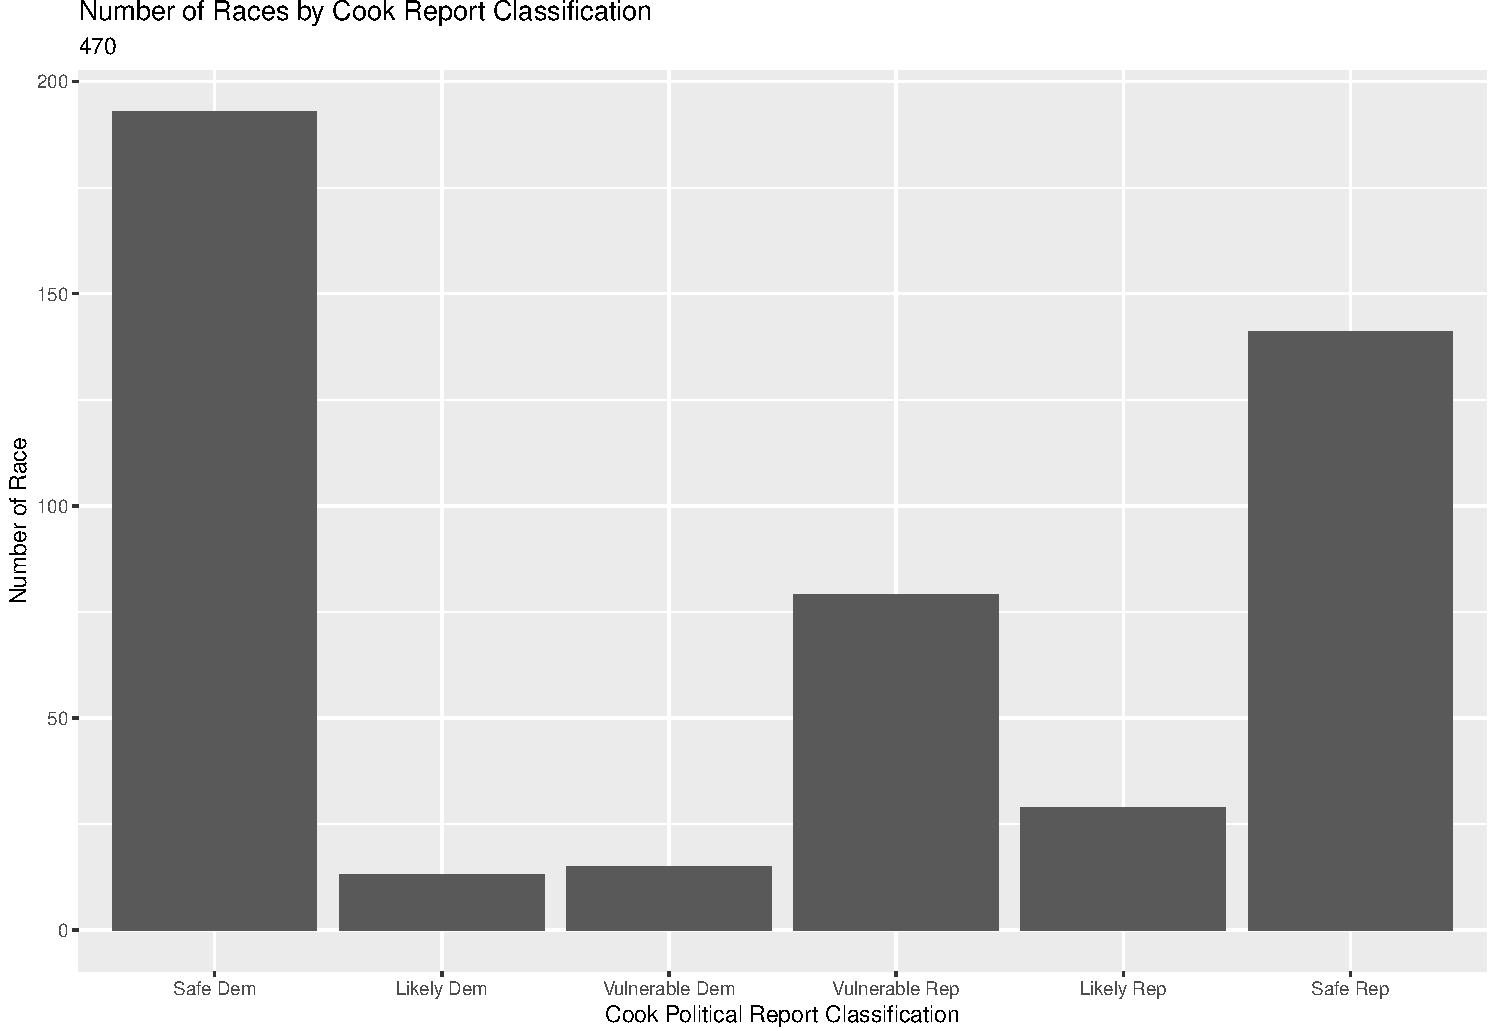
\includegraphics{final_files/figure-latex/class all-1.pdf}
\includegraphics{final_files/figure-latex/class all-2.pdf}

With that caveat in mind, we can now look at the predictive history of
our two tools over time. The chart below shows the probability of
democratic victory in our 120 races with the model probability plotted
on the x-axis and market price on the y-axis. This information is useful
when contrasted across time. The first chart shows the probabilities
from September 1st, while the second shows those from November 5th.
Highlighted in purple are races with an incumbent democratic candidate.
The skew of these races blow the \(x=y\) line shows a consistent
tendency for markets to underpredict the chances of these candidates
winning re-election compared to the forecasting model.

\includegraphics{final_files/figure-latex/plot diff-1.pdf}
\includegraphics{final_files/figure-latex/plot diff-2.pdf}

The difference in the two models over time is important due to the
different types of data incorperated in each tool at different points in
the campaign. FiveThirtyEight makes an effort to stress the importance
of polling in their model. More polling is done closer to the election,
theoretically improving the accuracy of the model. On the other hand,
the efficient market hypothesis states that the prediction markets
should always reflect all information available to the traders.
Forecasting models themselves are an important data point traders use to
calibrate their predictions. Closer to the election, the difference in
the two predictions decreases as the models gain strength and the
traders rely more on hard data and less on their gut.

The chart below shows the average difference in market price and model
probability over time for different types of candidates. You can see the
markets consistently undervalue the probability of Democratic incumbents
by roughly 10 points compared to the forecasting model. The chances for
Democratic challengers starts higher in the prediction markets, but dips
below the forecasting model over time. This chart is an important
diagnostic tool to assess the potential bias of the prediction markets.
In an interview with the Casino City Times, Brandi Travis, the chief
marketing officer for Aristotle (the company which opperates the
PredictIt website for the University of Wellington) admited that ``Most
of our users are between the ages of 21 and 39, and the majority are
male\ldots{}'' This kind of skew should not be an issues as it would be
with polling. Despite the potential political bias of traders, the
market forces of risk aversion and profit maximizing should incentivize
a apolitical trading. The consistent undervalue of incumbent Democratic
chances could signal market errors or a be legitimate difference in
opinion as to their electoral chances.

\includegraphics{final_files/figure-latex/diff time-1.pdf}

To analyze the accuracy of the predictions, I performed one last
relational join of the final tibble and the AP election results. For
each prediction, the candidate with a greater than 50\% probability is
the predicted winner. For every day, the predicted winner by each tool
was compared to the election results. An average of correct predictions
for each tool on every day was calculated and plotted over time. From
the graph below, we can see how the two prediction tools perform over
time. Among existing markets on August 10th, traders placed a greater
probability on the eventually winner in excess of 90\% of the time. On
that same day, the winner as predicted by the market was closer to 80\%
accurate. Over time, however, both tools converged closer to 88\%
accuracy the day before the election. This convergence might represent
an increased reliance on the forecast model in the trader activity. Over
time, the accuracy of the model improves as polling becomes more
frequent and polling is able to more accurately capture the opinion of
an increasingly decided electorate.

\includegraphics{final_files/figure-latex/plot accuracy-1.pdf}

I believe these results present a clear role for prediction markets in
future elections. Data journalists should consider the value of
occasionally mentioning the prices of prediction markets alongside the
numbers calculated by proprietary forecasting models. Prediction markets
move faster than than models, which rely on polling to be completed and
released before probabilities are updated. This speed is useful for
campaign operatives and national parties to interprate the efficacy of
strategies in real time. Furthermore, the accuracy of prediction markets
early in the campaign cycle suggests traders are better able to capture
the uncertainty of the far off election in the absense of more
quantitative information like polling or fundraising.

\section*{References}\label{references}
\addcontentsline{toc}{section}{References}

\hypertarget{refs}{}
\hypertarget{ref-becker08}{}
Becker, Bernie. 2008. ``Political Polling Sites Are in a Race of Their
Own.''
\url{https://www.nytimes.com/2008/10/28/us/politics/28pollsite.html?_r=1}.

\hypertarget{ref-camerer05}{}
Hsu, Ming, Meghana Bhatt, Ralph Adolphs, Daniel Tranel, and Colin F.
Camerer. 2005. ``Neural Systems Responding to Degrees of Uncertainty in
Human Decision-Making.'' \emph{Science} 310 (5754). American Association
for the Advancement of Science: 1680--3.
\url{http://www.jstor.org/stable/3842970}.

\hypertarget{ref-silver16why}{}
Silver, Nate. 2016. ``FiveThirtyEight.''
\url{https://fivethirtyeight.com/features/why-fivethirtyeight-gave-trump-a-better-chance-than-almost-anyone-else/}.

\hypertarget{ref-silver18how}{}
---------. 2018. ``How Fivethirtyeight's House, Senate and Governor
Models Work.''
\url{https://fivethirtyeight.com/methodology/how-fivethirtyeights-house-and-senate-models-work/}.

\hypertarget{ref-doi:10.1002ux2ffor.2339}{}
Vaughan Williams, Leighton, and David Paton. n.d. ``Forecasting the
Outcome of Closed-Door Decisions: Evidence from 500 Years of Betting on
Papal Conclaves.'' \emph{Journal of Forecasting} 34 (5): 391--404.
doi:\href{https://doi.org/10.1002/for.2339}{10.1002/for.2339}.


\end{document}
